\section{Error Propagation}

\subsection{Differential}
\begin{wrapfigure}{r}{6cm}
    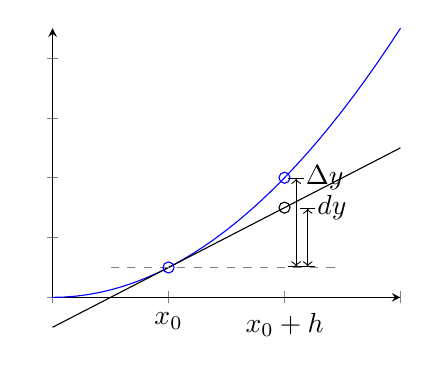
\begin{tikzpicture}
\begin{axis}[
    clip=false,
    width=6cm, height=5cm,
    axis lines=left,
    domain=0:2.5,samples=31,
    xmin=0, xmax=3,
    ymin=0, ymax=9,
    xticklabels={{},{},{$x_0$},{$x_0+h$},{}},
    yticklabels={},
]

    % Plots
    \addplot[domain=0:3,samples=31,blue,mark=none] {x^2};
    \addplot[blue,mark=o,only marks] coordinates {(1,1)(2,4)};
    \addplot[domain=0:3,samples=2,black,mark=none] {2*x-1};
    \addplot[black,mark=o,only marks] coordinates {(2,3)};

    % Labels
    \draw[dashed,gray] (axis cs:0.5,1) -- (axis cs:2.5,1);
    \draw[|<->|] (axis cs:2.2,1) -- (axis cs:2.2,3) node[anchor=west] {$dy$};
    \draw[|<->|] (axis cs:2.1,1) -- (axis cs:2.1,4) node[anchor=west] {$\Delta y$};

\end{axis}
\end{tikzpicture}
\end{wrapfigure}

The differential $df$ denotes the linear part of the increment of a variable in a function.
\[
    \Delta f = f(x_0+h)-f(x_0) \approx df = f'(x_o) dx = f'(x_0) h = f'(x_0) \Delta x
\]

$\Delta f$ is the \emph{absolute} error of $f$ at $x_0$.
The \emph{relative} error is $\frac{\Delta f}{f} \approx \frac{df(x_0)}{f(x_0)}$

Any $n$ times differentiable function can be approximated with a \textbf{Taylor} series:
$$f(x_0+h) = f(x_0) + h f'(x_0) + \frac{h^2}{2} f''(x_0) + \frac{h^3}{3!} f'''(x_0) +
\ldots + \frac{h^n}{n!} f^{(n)} + R_n(x_0,h)$$
Where $R_n(x_0,h)$ denotes the remainder term and converges to $0$ with a speed of $o(h^n)$ ("fast") as $n \rightarrow \infty$. There are, for example, the
\begin{align*}
    \text{Lagrange Form: } R_n(x_0,h) &= \frac{h^{n+1}}{(n+1)!} f^{(n+1)}(\underbrace{x_0 + \vartheta h}_{\xi})
    \qquad (\xi \in (x_0, x_0+h), \vartheta \in (0,1)) \qquad \text{or the} \\
    \text{Cauchy Form: } R_n(x_0,h) &= \frac{h^n(1-\vartheta)^n}{(n+1)!} f^{(n+1)}(\underbrace{x_0 + \vartheta h}_{\xi})
    \qquad (\xi \in (x_0, x_0+h), \vartheta \in (0,1))
\end{align*}

With the Taylor series, the absolute error becomes
\[
    \Delta f = \frac{1}{1!}df(x_0) + \frac{1}{2!}d^2f(x_0) + \ldots + \frac{1}{n!}d^n f(x_0) + R_n(x_0,h)
\]


\subsection{Multivariate Differentials, Taylor}
In the multidimensional case, the differential looks like this:
\[
    \Delta f \approx df(\vec{x}) = \sum\limits_{i=1}^n \frac{\partial f(\vec{x})}{\partial x_i} h_i = h_1 \frac{\partial f(\vec{x})}{\partial x_1} + \ldots +
    h_n \frac{\partial f(\vec{x})}{\partial x_n} \qquad \text{with} \quad \vec{h} = [h_1, \ldots, h_d]^T, \; \vec{x} = [x_1, \ldots x_d]^T
\]

The vector field of partial derivatives is called the gradient field of $f$ and is denoted by $\operatorname{grad}(f)$ or $\vec{\nabla} f(\vec{x})$.
Thus, $\Delta f \approx \vec{\nabla} f(\vec{x}) \cdot \vec{h}$.

In the multivariate case, the Taylor series for multi-indices $\alpha = \{ \alpha_1, \hdots , \alpha_n \}$ and $|\alpha| = \alpha_1 + \hdots + \alpha_n $ is given by
\[
    f(\vec{x}_0+h) = f(\vec{x}_0) + \frac{1}{1!}\vec{\nabla}f(\vec{x}_0) \cdot \vec{h}
    + \sum\limits_{|\alpha|=2}^N \frac{1}{\alpha!}\frac{\partial^{|\alpha|} f(\vec{x}_0)}{\partial x^{\alpha}} \cdot \vec{h}^{\alpha}
    + \sum\limits_{|\alpha|=N+1} R_{\alpha}(\vec{x}_0,\vec{h}) \cdot \vec{h}^{\alpha}
\]

or simplified for 2nd order
\[
    \begin{split}
        f(\vec{x}_0 + \vec{h}) = & f(\vec{x}_0) + \vec{h} \nabla f(\vec{x}_0) +
        \underbrace{\bigg( \frac{h_1^2}{2!} \frac{\partial^2 f}{\partial x_1^2} + \frac{h_2^2}{2!} \frac{\partial^2 f}{\partial^2 x_2^2}
        + \frac{h_1 h_2}{1!1!} \frac{\partial^2 f}{\partial x_1 \partial x_2}\bigg)}_{\text{for 2nd order}} + \\
        & R_{(3,0)}(\vec{x}_0, \vec{h}) \cdot \vec{h}_1^3 + R_{(2,1)}(\vec{x}_0, \vec{h}) \cdot \vec{h}_1^2 \vec{h}_2 + R_{(1,2)}(\vec{x}_0, \vec{h}) \cdot \vec{h}_1 \vec{h}_2^2 + R_{(0,3)}(\vec{x}_0, \vec{h}) \cdot \vec{h}_2^3
    \end{split}
\]

\subsection{Jacobian Matrix}
\begin{minipage}{12cm}
    The Jacobian matrix maps all first derivatives of a function.
    If the Jacobian matrix is square ($m=n$), its determinant $\det(J)$ can be interpreted as the transformed volume:
    \[
        \underbrace{dy_1 dy_2 \ldots dy_n}_{\text{"`transformiertes Volumenelement"'}} =
        \det(J_f(\vec{x})) \underbrace{dx_1 dx_2 \ldots dx_n}_{\text{"`Volumenelement"'}}
    \]
\end{minipage}
\begin{minipage}{6cm}
    \[
        J_f(\vec{x}) :=  \begin{bmatrix}
        \frac{\partial f_1}{\partial x_1}(\vec{x}) & \frac{\partial f_1}{\partial x_2}(\vec{x}) & \ldots & \frac{\partial f_1}{\partial x_n}(\vec{x}) \\
        \vdots & \vdots & \ddots & \vdots \\
        \frac{\partial f_m}{\partial x_1}(\vec{x}) & \frac{\partial f_m}{\partial x_2}(\vec{x}) & \ldots & \frac{\partial f_m}{\partial x_n} (\vec{x})
        \end{bmatrix}
    \]
\end{minipage} \\

The Jacobian determinant can also be a measure of error propagation.
The calculation is done directly using the determinant rule, or
$$\frac{D(f_1, f_2, \ldots,f_n)}{D(x_1, x_2, \ldots, x_n)} = \det(J_f(\vec{x})) \quad \text{or} \quad
\det(J_f) = \sqrt{\det \Big( \underbrace{J_f^T(\vec{x}) J_f(\vec{x})}_{\text{diagonal matrix}} \Big)}.$$

Also, for the transformation $T$ and its inverse $T^{-1}$: $\det(J_T) = \frac{1}{\det{J_{T^{-1}}}}$
\hspace{5mm}
